%!TEX root = ../report.tex
\chapter{Setting Up Automated Build}\label{chap:config_management}
Starting the first sprint we need to understand the systems given to us by previous semesters. We mainly look at setting up automated build, but also do some setup of the Redmine tool.

\begin{chapterorganization}
  \item in \sectionref{sec:redmine-conf} we describe how we customize Redmine to suit our needs;
  \item in \sectionref{sec:jenkins} we describe the platform for continuous integration, Jenkins, that we use in the project;
  \item in \sectionref{sec:build_automation} we explain how we set up automation of the builds and discuss version control branching strategies as well as automated testing and lint checking;
  \item in \sectionref{sec:automated_documentation_gen} we explain how we set up automated documentation generation.
\end{chapterorganization}

\section{Configuring Redmine}\label{sec:redmine-conf}
The developers of last year used Redmine for various project management functions, and we need to evaluate which of the functions to keep. One of these functions is an issue tracker which we choose to keep, but not as a traditional issue tracker. We customize it to contain the product backlog and release backlog. Redmine is not an ideal tool for this purpose, as the workflow of adding and updating tasks is slow and tedious. However it is what the multi-project has available without additional effort. We collaborate with the Redmine and issue tracker groups. We specify how user stories should be handled in Redmine, and the aforementioned groups implement the changes.

Also, a Gantt chart feature had been installed by previous years. The Scrum method does not advocate Gantt charts or other dependency charts \parencite{larman2003}. As such, we collaborated with the Redmine group to remove this from Redmine. The other unused features have not been removed, since it was deemed unnecessary to spend time on doing so.

Redmine also contains other features such as a roadmap, burndown charts, and news. While these features are present on the main page, they are not used. The burndown chart in particularly is not used since no common sprint backlog is used, and as such the burndown chart cannot be used at the multi-project level.

We initially used Redmine as Scrum board within our group, but due to Redmine being very slow and tedious to update, we replace it with a physical Scrum board.

\section{Jenkins: Continuous Integration Platform}\label{sec:jenkins}
An open source tool for continuous integration, Jenkins \parencite{JenkinsWebsite}, was used by previous years. We will continue to use this as our continuous integration platform. It supports source control management tools such as Git \parencite{gitwebsite}, as well as build automation tools such as Maven \parencite{mavenwebsite}. It is extensible via numerous available plugins. Jenkins allows for a sophisticated continuous integration setup, however the setup by previous years is rather basic and we want to improve it in several ways.

\subsection{Upgrading Jenkins and Plugins}
We inherit the old installation which has not been updated in a long time. Jenkins itself and all the Jenkins plugins have updates available. We update everything to the newest versions.

\subsection{Setting up Roles in Jenkins}
The inherited Jenkins installation is open to anybody. We do not find this sensible as we need to control the build process. Allowing everybody access will likely end in someone modifying a setting without our knowledge. Because we set up a mechanism for automatic build, other people do not need the option to start builds manually. It might even interfere with the automatic build, if other people have access to the Jenkins configuration.

It is important that everyone can see the build process, however. According to Martin Fowler, it is important that everyone is able to see the state of builds and which parts of the overall system that are currently worked on \parencite{fowlerCI}. In addition to this, we find it important that developers can follow the testing process of their new code, and how stable different projects are. This way, we are able to transfer human resources between code bases if needed, and it may work as a motivation for the developers to create stable builds. Because of this, we give developers read-only access to Jenkins, while we are the only people with write access.

\section{Build and Test Automation}\label{sec:build_automation}
The inherited project has no build automation. As a part of the automated build and deployment story, we want to be able to build the code automatically, and even continuously. We decide to set it up in two stages. In Jenkins each build process configuration is organized into an entity called a job. Each app that is build with Jenkins has a Job that defines the steps needed to build that app. In the first stage we schedule all jobs to run nightly. This gives us some level of build automation and gives us time to investigate merge strategies and set it up properly. The nightly job is set to run every day at midnight.

\subsection{Merge Strategy}\label{sec:branching_strategy}

\begin{figure}
\begin{subfigure}[b]{\linewidth}
\centering
\tikzsetnextfilename{mergestrategy}
\begin{tikzpicture}
% MASTER
\node[text width=2cm] at (0,1) {\mono{master}};
\node(master_a) [draw, circle, minimum size=0.5cm] at (2,1) {\mono{A}};
\node(master_head) [draw, circle, minimum size=0.5cm] at (5,1) {\mono{D}};
\node(master_head_label) [] at (5,2) {\mono{HEAD}};
\draw[->, >=latex] (master_head) -- (master_a);
\draw[->, >=latex] (master_head_label) -- (master_head);

% LOCAL
\node[text width=2cm] at (0,0) {\mono{dev\_branch}};
\node(local_b) [draw, circle, minimum size=0.5cm] at (3,0) {\mono{B}};
\node(local_c) [draw, circle, minimum size=0.5cm] at (4,0) {\mono{C}};
\draw[->,>=latex] (local_b) -- (master_a);
\draw[->,>=latex] (master_head) -- (local_c);
\draw[->,>=latex] (local_c) -- (local_b);
\begin{pgfonlayer}{background}
  \filldraw [line width=4mm,join=round,black!10]
      (-1, 1.2)  rectangle (6,0.8)
      (-1, 0.2)  rectangle (6,-0.2);
\end{pgfonlayer}
\end{tikzpicture}
\caption{The direct commit strategy}\label{fig:commit_stratagy_a}
\end{subfigure}\\
\begin{subfigure}[b]{\linewidth}
\centering
\begin{tikzpicture}
% MASTER
\node[text width=2cm] at (0,2) {\mono{master}};
\node(master_a) [draw, circle, minimum size=0.7cm] at (2,2) {\mono{A}};
\node(master_head) [draw, circle, minimum size=0.7cm] at (6,2) {\mono{D}};
\node(master_head_label) [] at (6,3) {\mono{HEAD}};
\draw[->, >=latex] (master_head) -- (master_a);
\draw[->, >=latex] (master_head_label) -- (master_head);

% PENDING HEAD
\node[text width=2cm] at (0,1) {\mono{intermediate}};
\node(ph_head) [draw, circle, minimum size=0.7cm] at (5,1) {\emph{\mono{I}}};
\draw[->, >=latex] (master_head) -- (ph_head);

% LOCAL
\node[text width=2cm] at (0,0) {\mono{dev\_branch}};
\node(local_b) [draw, circle, minimum size=0.7cm] at (3,0) {\mono{B}};
\node(local_c) [draw, circle, minimum size=0.7cm] at (4,0) {\mono{C}};
\draw[->,>=latex] (local_b) -- (master_a);
\draw[->,>=latex] (ph_head) -- (local_c);
\draw[->,>=latex] (local_c) -- (local_b);

\begin{pgfonlayer}{background}
  \filldraw [line width=4mm,join=round,black!10]
      (-1, 2.2)  rectangle (7,1.8)
      (-1, 0.2)  rectangle (7,-0.2);
  \filldraw [line width=4mm,join=round,black!10]
      (-1, 1.2)  rectangle (7,0.8);
\end{pgfonlayer}
\end{tikzpicture}
\caption{The pre-tested commit strategy}\label{fig:commit_stratagy_b}
\end{subfigure}
\caption[Different branching strategies]{Different branching strategies. A circles represents a commit and an arrow represents a reference to a commit.}\label{fig:commit_stratagy}
\end{figure}

As the name \emph{continuous integration} suggests, code should be integrated into the mainline (or \emph{master branch}) of the project frequently \parencite{fowlerCI}. According to Martin Fowler, frequent merges ensure that merges generally will be small and easy to perform \parencite{fowlerFeatureBranch}. The master branch must be stable and always in a release-ready state. If it breaks, it should be the team's first priority to fix it. A consequence of this is that the whole team is affected when a developer introduces an error, which has a negative influence on the overall productivity.

We assess two strategies to accommodate these consequences of continuous integration: A \emph{direct commit strategy} and the \emph{pre-tested commit strategy}. In the direct commit strategy \parencite{git_branching_workflows2015}, every developer integrates their code directly to the master branch. It is the developer's own responsibility that the code works. This is the simplest, and one may say, the most agile way of integrating code with the master branch. An illustration of the direct commit strategy can be seen in \figureref{fig:commit_stratagy_a}. A developer creates a branch from the master branch and develops their code (commits \mono{B} and \mono{C}) on this before merging it directly into the master branch (commit \mono{D}).

An alternative to integrating code directly with the master branch is to use pre-tested commits \parencite{fowlerPendingHead}. A pre-tested commit uses a special branch which is an intermediate place for building and testing code before it is merged into the master branch. The code will only be merged into the master branch if it passes the tests. This ensures that the master branch will always work, but the merging workflow will be more complex as the developer must pull from one branch and push to another. The strategy is illustrated in \figureref{fig:commit_stratagy_b}. The developer creates a branch from the master branch and develops its code on here. When completed, the code is merged with the intermediate branch (commit \emph{\mono{I}}), which will build and test the code before eventually merging it with the master branch (commit \mono{D}).

For the first sprint, we choose to implement the direct commit strategy, primarily because of its simplicity. It is important to get continuous integration up running so the developers can start to develop code, and it would be too costly to spend time implementing a pre-tested commit strategy as this will block the progress of all other developers. We are unsure about how the developers handle the increased responsibility, so in the preparation of the second sprint, we will evaluate this strategy and consider whether we should implement the pre-tested commit strategy instead.

\subsection{Continuous Build and Deployment}\label{sec:auto_deploy}
We want a build job to be started automatically when changes are made to the code. We do this by setting up a post-receive Git hook that invokes Jenkins. Jenkins then automatically builds jobs that have code pushed to their master branch. The hook can be seen in \listingref{lst:hook_script_first}. \code{curl} sends an HTTP GET request to Jenkins with the needed information to start a build on a job associated with a particular repository. \mono{http://cs-cust06-int.cs.aau.dk/git-ro/\$(basename \$(pwd))} is the link for the repository to update. Since we use the same Git hook script in all repositories, and there are several repositories, the name of the repository that invokes the hook is found by \code{\$(basename \$(pwd))}. Finally a message is displayed to the user that pushed to tell them that Jenkins will start building.
\begin{lstlisting}[language=bash,showstringspaces=false,caption=Git hook bash script,label=lst:hook_script_first]
curl -s http://localhost/jenkins/git/notifyCommit?url= http://cs-cust06-int.cs.aau.dk/git-ro/$(basename $(pwd)) > /dev/null

echo "Thank you for your push. Jenkins will be serving you in a moment."
\end{lstlisting}

In Jenkins there is a job called \emph{deployment} which builds all other jobs and moves the APKs to a specific directory. An APK file is the output of a build and is a package format used to distribute and install software onto Android. We remove this job and make it a part of the build process of every job to do this themselves, and ensure there are no redundant APKs present in the APK directory. By making it a part of every job we also ensure that there always is an up-to-date version of all applications whenever they pass a build, complementing our vision for continuous integration. This additional work was unplanned, and we do not have time to set it up on all jobs in this sprint.

\subsection{Continuous Test}
\label{sec:test_automation}
Now that the automatic test setup is created, we examine the different types of automatic tests we can use on Android.

Because one of the ideas behind automated build is to give the developer fast feedback on the state of the code, the build and test process should be fast. The Extreme Programming (XP) development method states 10 minutes as a guideline for how much time a build should take \parencite{beck2004}. While we think this is a reasonable time, not all parts of the system can be thoroughly tested in that time. In such cases, Martin Fowler suggests that the fastest and general tests should be whenever a commit is pushed to the master branch, and slower tests can be triggered for later execution \parencite{fowlerCI}. We call these kinds of tests \emph{delayed tests}.

\subsubsection{Unit Testing}
During the initial investigation of the inherited code base we found some existing unit tests in one of the GIRAF apps. The unit tests runs in an emulated Android environment, or on actual Android devices if any are connected to the computer. These tests utilize the Android unit testing framework included in the Android framework \parencite{AndroidUnit}. We decide to postpone any further investigation into unit testing frameworks. Instead, we focus on getting the existing unit tests to run, both locally and in Jenkins. The tests were immediately runnable through Android Studio 0.4.6. However, Android Studio does something behind the scenes when it runs the tests, and therefore we cannot run them from the command line, which means that we cannot run them in Jenkins. However, the most recent Android studio, version 1.0.2, uses Gradle exclusively to run the tests. This means that when the apps are migrated to the new version, we are able to run the tests with Jenkins. The other GIRAF apps did not have any tests, so we create test projects, with examples of tests to verify that Jenkins can run the tests. This makes it easier for the other groups to start writing tests, as there is then a unit testing framework in place, as well as an example test.

Currently, Jenkins starts a new emulator for testing before each project is built. This adds a significant delay to the build. The building time when building all apps has increased from 20 minutes to 90 minutes. This is unfortunate, but for now we will not spend more time improving this. We may return to this in a later sprint. Unit tests are the simplest tests we have, and we do not want these to be handled as delayed tests. Because of the slow emulator startup, we only start a single emulator. This means that apps are tested only on a single Android device configuration, which in turn means that we may not discover all errors when testing. However, it is better than no testing and we may expand the range of devices in the future.

\subsubsection{UI Testing and Monkey Testing}
Because Android applications contain a graphical user interface, it is not sufficient to only test the backend libraries. On the overall level, there are two ways of performing automatic testing of the user interface in Android: UI testing and monkey testing. UI testing is a way of declaring specific sequences of events and their expected behaviors. For example, a test may specify a click on a settings button and assert that this actually opens the settings screen. Writing UI tests can be labor-intensive, though, and the maintenance of the tests can get quite comprehensive. As an alternative, monkey testing can be used. Monkey testing is performed by inputting a random sequence of events, such as buttons clicks and touches, into a device. That way, the user interface of an app is randomly tested. There are no guarantees that all parts of the app will be tested, but the setup of the test is generally simple. The official Android SDK has monkey testing facilities built in, and there exists a Jenkins plugin for running these. Because of the simplicity of monkey testing and because the GUI application developers have requested this as a tool for discovering bugs in the code, this is the way we automatically test the user interface. We plan to make Jenkins run monkey tests during the night, as delayed tests, when the server is otherwise idle.

While the Android monkey tool can test multiple applications at once, the Jenkins plugin does not support that feature. The monkey test command can take as an argument a number of packages (apps) to test, using the \code{-p} option, for example \code{monkey -p package1 -p package2 -p package3}. The Jenkins plugin does not support making more than one \code{-p} option. The plugin is open source, so we add support for this feature, by contributing code\footnote{Commits on Github (\url{https://github.com/jenkinsci/android-emulator-plugin}): \href{https://github.com/jenkinsci/android-emulator-plugin/commit/71385cfb3e3bb4dfa6d11170c52ee69808a4f72f}{71385cf},  \href{https://github.com/jenkinsci/android-emulator-plugin/commit/811bfac657565b25ce2f7fc9d6399d9f22bb6042}{811bfac}, \href{https://github.com/jenkinsci/android-emulator-plugin/commit/5395bb1fd23032cab48a7bfff61a26544f078785}{5395bb1}}. Multiple packages are now delimited by comma. The reason for this is that we found that some users of the plugin exploited the way the package name was inserted as an argument to the monkey tool in order to insert different arguments. Because a comma character is not used in any argument to the monkey tool (compared to for example a whitespace character), we expect that no existing users will be affected by the change.

Additionally, the plugin requires the tested apps to be installed. However, we do not have the APKs of all apps easily available. Therefore we do not manage to setup monkey testing in this sprint.

\subsubsection{Concolic Testing}
Concolic testing is a way to statically analyze code in order to find bugs, e.g.\ potential null pointer exceptions. Concolic testing uses a combination of symbolic execution and testing of particular paths in order to maximize code coverage \parencite{concolic_testing_2015}.

To our knowledge, the only framework for concolic testing that works with Android projects is \emph{Acteve} \parencite{AnandNHY12, AnandH11}. The documentation for this framework is non-existent, and we cannot find anything except for an unsuccessful attempt to build and run Acteve \parencite{chenxiong-acteve}.

We already have unit testing and many crash reports to occupy the time of many multi-project groups, and as such we do not think concolic testing is worth the payoff, so we will not spend more time investigating this.

\subsection{Automated Lint Check}\label{sec:automated_lint}
Lint checking is static code analysis that scans the source code for potential bugs and improvements. We investigate the possibility of automating lint checks on the source code, as we suspect this will uncover a wide range of improvements.

An official tool, Android Lint \parencite{AndroidLint}, for linting Android project source files exists. It checks for potential bugs and optimization improvements for correctness, security, performance, usability, accessibility, and internationalization.

There are some important considerations when choosing to lint the source code automatically. The code base is inherited from earlier years and no lint checking to our knowledge was performed on this. Linting the code will produce a considerable amount of warnings. It is therefore not possible for us to let a build fail if it contain any warnings.

We set up automated lint checking in Jenkins on all jobs. The warnings are presented in the build overview screen, as seen in \figureref{fig:jenkins-overview}. We hope that having a low number of lint warnings will be incentive enough for each group to fix warnings.

\begin{figure}[htbp]
    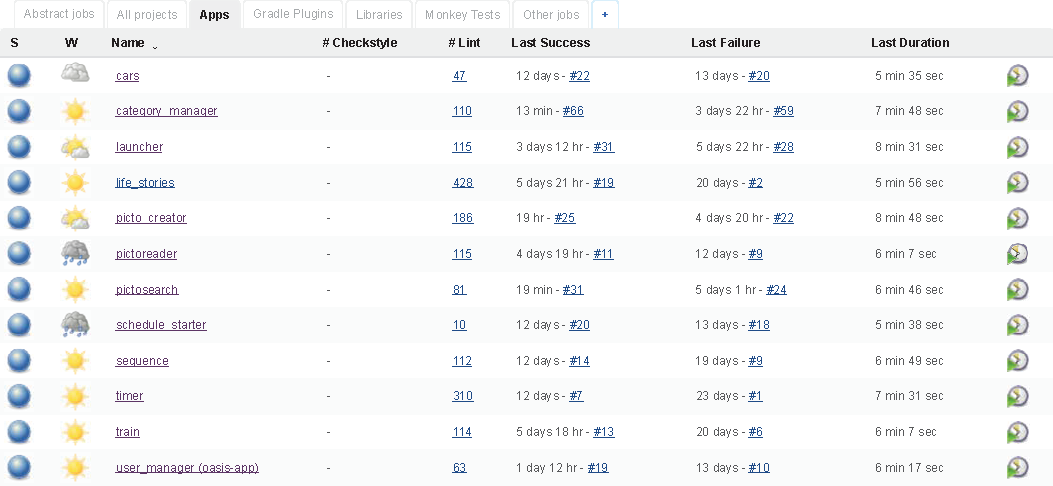
\includegraphics[width=\textwidth]{graphics/jenkins-overview.pdf}
    \caption{Screenshot of a section of the build overview screen, which shows the lint warning column}
    \label{fig:jenkins-overview}
\end{figure}

Over time, we hope that the presence of serious lint warnings can be a reason to fail a build. We may adopt this practice in a later sprint, and to help speed up this adoption we may set it up as follows. As there are a large number of lint warnings already in the code, a baseline day can be selected. Groups should not be \emph{punished} (i.e.\ the build fails) for lint warnings that were present before the baseline day. Only newly introduced lint warnings should be considered and punished.

\section{Automated Documentation Generation}\label{sec:automated_documentation_gen}
When working with a large code base, people will most likely not have insight in all parts of the code. Some kind of documentation is helpful in order to know how to use libraries. However the agile manifesto states that one should prioritize working code over documentation \parencite{agile-manifesto-web}. Therefore we do not intend to write comprehensible documentation of the code. A consequence of being agile is that the system architecture is likely to change rapidly --- so it is important that little effort is required for updating the documentation. To make the documentation easy to find, we want the documentation for all projects accessible from one place. Based on these requirements, we choose to use a documentation generator which automatically generates documentation from the code rather than writing such documentation manually. The documentation will not be all-encompassing, but act more like a guide to the code.

We investigate the Javadoc \parencite{javadoc} and Doxygen \parencite{doxygen} tools. Both tools are cross-platform and can be integrated with Jenkins. Javadoc can generate documentation in HTML and Doxygen can generate both HTML and \LaTeX. We will generate HTML documentation which will be hosted on the server.

Javadoc is the official documentation generator for Java and generates documentation based on specially formatted comments embedded in the source code. This format is integrated in Android Studio, making the documentation easily accessible where needed. In addition, parts of the existing code already contain Javadoc comments. A problem with Javadoc, however, is that it follows the packages and classes referred in a Java file. A requirement for this is that the source code must be a correctly structured Java project in order for the tool to find the different classes. This makes it complicated to comply with the requirement of having documentation of all projects in one place, because a combination of all projects may not form a valid Java project. The source code of all projects cannot simply be copied into one directory and fed to the Javadoc tool.

The Doxygen tool is a cross-language documentation generator that supports the same documentation syntax as Javadoc. Doxygen does not follow the class dependencies but simply parses the specified files. The HTML-documentation is very similar to that of Javadoc, and because it is more convenient to use, we have chosen to use this tool for documentation generation.

\subsection{Documentation Generation in Jenkins}
We have configured a Jenkins job to generate the documentation for all projects. This job pulls the most recent state of the master branch of each project and executes the Doxygen tool on all code. On the current code base, the doxygen tool uses up to 7 minutes to generate the documentation because of the size of it. Because we do not want to block more important jobs, such as building and testing new commits, we choose to run this job nightly.